\documentclass[12pt]{article}

\usepackage[T3]{fontenc}
\usepackage[utf8]{inputenc}
\usepackage[russian]{babel}

\usepackage{graphicx}
\usepackage{mhchem}

\usepackage{gensymb} % degree symbol
\usepackage{nicefrac} % nice fractions
\usepackage{mathtext}

\usepackage{titling}

\title{Определение удельной энтальпии сгорания бензойной кислоты.}
\date{}

\newcommand{\tn}{\textnormal}
\newcommand{\vlevo}{\hspace*{-0.63cm}}

\setlength{\droptitle}{-11em}

\begin{document}

\maketitle

\vspace*{-3cm}

\begin{figure}[!h]
  \centering
	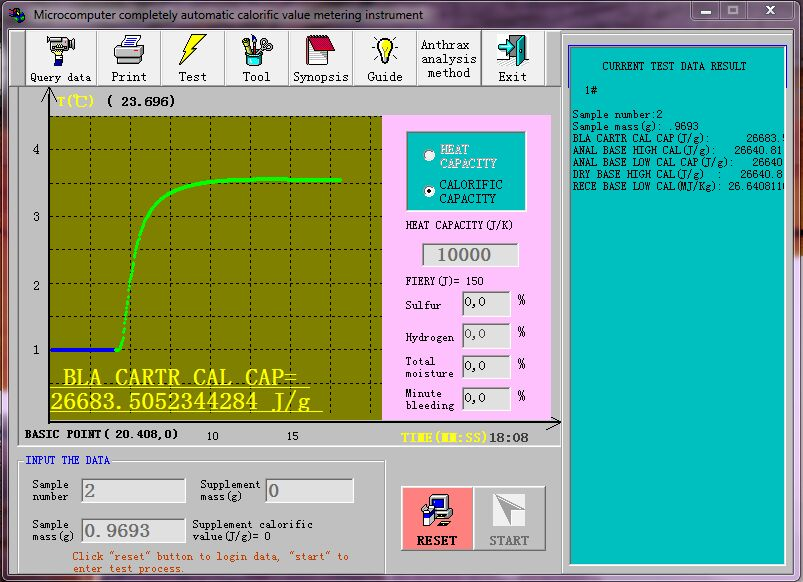
\includegraphics[width=\textwidth]{Plot.jpg}
	\caption{График температурной зависимости.}
	\label{fig:Temperature}
\end{figure}

Полученное значение энтальпии сгорания бензойной кислоты: \( \Delta H_{\tn{сгор.}} = 26.68 \, \nicefrac{\tn{кДж}}{\tn{г}} = 3255.44 \, \nicefrac{\tn{кДж}}{\tn{моль}}\). \\
Литературное значение энтальпии сгорания безнойной кислоты: \( \Delta H_{\tn{сгор.}} = 3226,7 \, \nicefrac{\tn{кДж}}{\tn{моль}} \).

\end{document}